\chapter{Head To Toe 1}

% \begin{figure}[H]
%     \centering
%     \includegraphics[width=\textwidth/2]{./Games/EveryChildCanSucceed/Images/EveryChildCanSucceed1CD.png}
%     \caption{Every Child Can Succeed 1 CD}
% \end{figure}

The first of the Head To Toe games published and released by The Lightspan Partnership for the PlayStation 1.

Head To Toe 1 features four video programs:

\begin{itemize}
    \item In the Beginning
    \item Cells\dots Your Starting Place
    \item In a Heartbeat
    \item Muscles\dots Holding You Together
\end{itemize}

\clearpage
\newpage

\section{In the Beginning}

\subsection{Audio Summary}

"In the Beginning" discusses how human and animal babies develop.

\subsection{Transcription}

Joy: This is the beginning of the show.

Boy 1: This caterpillar's the beginning of a butterfly.

Joy: This is the beginning of the alphabet.

Christopher: These seeds are the beginning of flowers.

Sarah: This pine cone is the beginning of\dots Um\dots The beginning of a tree!

Christopher: These tadpoles are the beginning of frogs.

Bob: Are you beginning to get the idea? That's what we're going to talk about on this show: Beginnings, especially the beginnings of things that are alive like animals and people. People like you guys and you. And here's a good place to start: okay, who knows what this is the beginning of?

Joy: A bird?

Bob: A bird.

Sarah: Chicken!

Bob: Chicken, yeah.

Christopher: Breakfast!

Bob: Well, this one's not going to become breakfast, Christopher, because inside it there's a chicken. An egg doesn't look like much on the outside, but inside, that chicken's waiting to be born. Now you guys already knew that, right? And that's because we've been watching chicks hatch from their eggs in our incubator. Let's have a look.

Bob (voice over): The egg is like a little house protecting the unborn bird. Inside of it, there's enough food to help the chicken grow and grow until she's strong enough to break through the shell. It takes her a little while, but soon she's free and ready to see the world.

Bob: Okay, [I see]\dots Yeah, boy this guy's pretty tired, he just came out of the egg.

Joy: Yeah, we saw him.

Sarah: [We saw the] one that's quiet.

Bob: One that's quiet?

Sarah: This one's quiet.

Bob: Okay, let's see if we can get this guy out for you here. Here, hold your hand up. Hold your hand up.

Joy: This one's trying to get out.

Bob: Here he is.

Joy: This one's trying to get out.

Bob: Yeah, there's one being hatched right there. Okay, hold on to him. Just hold him up. Here, I'll take this guy here.

Sarah: One has red on him.

Bob: [Red on him]? What's it feel like? What's it feel?

Sarah: Warm.

Bob: Yeah, they're warm, aren't they? Yeah, yours has got the feathers coming up. It's getting kind of fluffy, isn't it? He's looking more like a chicken. Mine's still kind of wet, just came out of the egg. Isn't this amazing? These chicks are only a few minutes old. Just a little while ago, they were inside an egg. Well, let's put them back inside the incubator so that they'll stay warm and their feathers will fluff up and they'll turn into chickens. Can you name any other birds besides chickens?

Sarah: Robin!

Bob: Robins.

Christopher: Eagles.

Bob: Eagles, yeah.

Joy: Ducks?

Bob: Duck, yeah.

Christopher: Goose?

Bob: Goose, that's a big one. Yeah.

Sarah: Joey!

Bob: Joey! Joey? Who's Joey?

Sarah: My, my parakeet.

Bob: Ah, your parakeet. Another bird. And all of those birds are really different, aren't they? Some are really big like eagles and geese, and some are really small like robins. But they all had their beginnings in an egg. Okay, here's another question for you. Here's somebody you might recognize.

Children Together: Gurtrude!

Bob: Yeah, hi, Gertie. This is Gertrude the guinea pig. Hi, Gertie. He's talking to us too. Yes, say hello to Gurtrude.

Sarah: Can we pet him?

Bob: Sure. Hi Gurtrude. Now where do you think Gertrude came from? Hmm\dots

Christopher: The store.

Bob: Well, yeah, she may have - we did get her at the pet store, yes. But where do you think she was born? Do you think she came out of an egg?

Joy: I don't know.

Christopher: Tell us.

Bob: Well, some animals aren't born from eggs - they're born by coming directly out of their mother's body, and it's an amazing thing to watch. Would you guys like to see an animal actually being born?

Children Together: Yeah!

Bob: Sure. Here, here's a film of a baby whale being born. It came directly out of its mother's body - her mother's name is Shamu, and she was born at SeaWorld. Let's watch.

(Video plays)

Bob: Wasn't that wonderful? And it's amazing how that baby whale was born right out of its mother's body. You know something else? That is how you and you were born as well.

(doorbell rings)

Children Together: I'll get it.

Sarah: Hi, Monica.

Monica: Hi, guys. Got anything to eat?

Bob: Hi, Monica. Come on in.

Monica: I'm already in, Bob.

Bob: Oh, yeah, right. Well then, uh, have a seat. I asked Monica to come here today because, well, she's a lot of fun, but also because today she's got something to tell us.

Monica: And great news, guys. I'm going to have a baby.

Joy: No, you're not!

Monica: Pardon me?

Joy: You're not going to have the baby.

Monica: That's funny. I was sure I was.

Bob: Why don't you think Monica's going to have a baby, Joy?

Joy: Because when my mom was going to have a baby, she had a really big tummy.

Monica: Oh, I see. You don't think my tummy's big enough to have a baby inside, right?

Joy: Yes.

Monica: I think I can explain, but um, could I have an apple first?

Bob: An apple? Uh, yeah, sure.

Monica: Joy, do you know how a baby begins?

Joy: No.

Monica: Well, it's really cool. A baby begins as a special cell that's made by a mom and a dad, and it lives inside the mother's body. And it's really little, just like that freckle on your nose. And that's how you began, as a special tiny little cell inside your mother's body.

Christopher: What happens to it?

Joy: Well, Christopher, it begins to grow. It becomes two cells and then four cells, and pretty soon\dots Well, here, let me show you. I went to my doctor today, and he gave me these really neat pictures. See, after a few weeks, that tiny cell grows into this. That's an embryo, and that's what's inside of me right now, Joy. An embryo. And I haven't gotten big yet because the embryo is still really small. See, it's only about as big as my thumb, and it's right here inside me. And it keeps growing and getting bigger and bigger every day.

Joy: Will you get a big tummy?

Monica: Don't worry, I'll get enormous!

Bob: Oh, Monica, here's your apple.

Monica: Thanks. Um, could I have some peanut butter on that?

Bob: Peanut butter? On the apple?

Monica: Mhm.

Bob: Okay.

Monica: Thanks, buddy. So anyway, this embryo, it begins to grow, and after a while, it looks like this.

Sarah: It looks like a little person!

Monica: Doesn't it? We can see its itty bitty feet and hands and head. See, now it's called a fetus - that's spelled F-E-T-U-S, fetus. And that's what we call a baby before it comes out of its mother.

Christopher: How does the fetus get food?

Monica: Well, it just orders out for pizza.

Christopher: No, it doesn't.

Monica: Okay, okay, you're right, it doesn't order out for pizza. As a matter of fact, it doesn't even eat with its mouth yet. See, the fetus has a very special way of eating.

Joy: How's that?

Monica: Well, this may sound a little strange, Joy, but uh, do you have a belly button?

Joy: Yes.

Monica: Well, that's how a fetus gets its food. Right through its belly button.

Christopher: Huh uh!

Joy: That's not true.

Monica: No, it's true. Here, look. I have another picture to show you. See, there's a tube that comes from the mother and goes right into the belly button of the fetus. And through that tube goes all the food and oxygen that the fetus needs to grow. That's why I've been so hungry these days, you see, 'cause I'm not just eating for myself. I'm also eating for the baby because everything I eat goes through the tube to the baby so it can keep growing.

Bob: Well, Monica, here is your apple and peanut butter.

Monica: Great. You know, I would really love a pickle.

Bob: A pickle? With the peanut butter and apple?

Monica: What's wrong with that?

Bob: Nothing.

Christopher: How long does the fetus stay inside you?

Monica: Well, from the time that special cell begins to grow to the day the baby is born is about 9 months. But then when the fetus is big enough and strong enough, it comes out. Tada! The baby's born. Oh gosh, listen guys, I'm sorry I have to go. My husband and I decided that we would go swimming every day so that I could stay healthy for the baby, but I'll see you guys again real soon, okay?

Children Together: Bye Monica. See you.

Bob: Okay, Monica, here's your pic-kles. She left? Uh, what, what did I miss?

Christopher: Sit down, I'll tell you.

Christopher (voice over): You began as a special cell. It's made by your mom and your dad, and it lives inside of your mother's body. The cell grows and grows and becomes an embryo, and then a fetus with tiny feet and hands. In 9 months, you're born. Every part of you is very small except for your voice.

Bob: And that's how human life begins. But what happens then? Can a baby take care of itself after it's born? Well, not really. Babies actually need a lot of help. And you might know this if you've ever watched animal babies after they're born.

(video plays)

Woman (voice over): You're brand new and you're pretty helpless too. Not too much that you can do 'cause you're the baby. Oh, you can babble, you can coo, people tell you coochie coo. Why do they act the way they do? 'Cause you're the baby. In the middle of the night, no one gets uptight, when you tell them with no ifs, ands, buts, or maybes. You're not crying to be rude, but you really want some food. That's the way it goes when you're the baby. So if you babble, bay, or bark, and if you're frightened of the dark, just remember this remark and someday maybe you might be a proud mom or dad. It might be hard, but you'll be glad. So don't forget the fun you had just 'cause you're the baby.

(back to house)

Joy: Bob, we have a baby at our house now.

Bob: Oh, that's neat. Is it a baby boy or a baby girl?

Joy: It's a girl and its name is Laura.

Bob: Do you help take care of Laura?

Joy: Mhm, everybody does.

(video plays)

Joy (voice over): Laura sits in a swing and Mom straps her in so she won't fall out. All of her toys are soft so she won't get hurt when she plays with them.

Joy: Laura\dots Laura\dots

Joy's Mom: Okay honey, I think it's time to feed the baby now.

Joy: May I help?

Joy's Mom: Certainly.

Joy: She's so cute.

Joy (voice over): Laura needs a lot of food and a lot of love. Today we're going to Grandma's house. When Laura rides in the car, she needs a lot of protection. She's so little she can't do much yet, but soon she'll be old enough to ride bikes and play with me, and I can't wait.

(back to house)

Bob: And I'm sure you're going to have a great time with your little sister Laura as soon as she learns how to take care of herself, right Joy?

Joy: Right.

Bob: Yeah. We all have families, and we would like to show you what our families look like. We've made some drawings. Would you like to see them? Joy, why don't you go first and show us your picture?

Joy: Okay. This is my dad, my mom, my baby sister Laura, my brother [Arneil], and me.

Bob: That's great. Sarah, what's your family look like?

Sarah: My mom and dad and me and [Mary Ellen] and Zach and Peter and [Kate].

Bob: It's a pretty big family. Christopher, what's yours like?

Christopher: My mom, me, and my dog Ralph.

Bob: Ralph looks pretty big there. And this is my family: my parents, I've got two sisters, a brother, and me. I'm the tallest. I think I'm also the best looking. Don't you?

Children Together: No?

Bob: Well, all right.

Sarah: Why don't we pin our drawings up on the fridge?

Bob: Okay, that's a good idea. Why don't you guys go do that? And so we've seen how a baby begins - how a very tiny but very special cell inside the mother's body becomes an embryo, then it grows into a fetus, and about 9 months later, the baby's born right out of the mother's body. And Joy showed us how a newborn baby needs to be protected and cared for. I'm sure there's someone who protects and cares for you too. Well, I think it's time to put my picture up on the refrigerator. You know, guys, I still think that I'm the best looking member of my family, you know, don't you?

Children Together: Eeh!

Bob: Don't you? No? Well, all right. Well, I'm going to put it right there. And so our program on beginnings has finally reached\dots

Everyone Together: The end!

\subsection{Credits}

Footage Provided by: Baxter Communications, Methodist Hospital (Indianapolis), Ralston Purina, SeaWorld, Studio Link Inc;
Special Thanks to: Lis Daily Home, Rose Acre Farms, Wayport Pet Supply;
Models Donated by: Frey Scientific Inc, Denoyer-Geppert Science Company;

\section{Cells\dots Your Starting Place}

\subsection{Audio Summary}

"Cells\dots Your Starting Place". This segment covers the parts and functions of a cell, genetic traits, and the importance of good health.

\subsection{Transcription}

Bob: Hi. The kids are busy making some kind of big picture.

Girl 1: It's not just a picture, it's a mosaic!

Bob: A mosaic? What's that?

Girl 1: It's when you use a lot of little things to make one big thing. See, we're using little pieces of paper.

Bob: Oh, I get it. So you guys are putting together these little tiny pieces of paper\dots

Boy 1: And when it's done, you get one gigantic picture.

Bob: Oh, so what's the picture of?

Girl 2: We're not telling!

Bob: Oh, come on.

Children Together: Go away!

Bob: Oh, oh, okay, okay, okay. I won't look, I won't look.

(move to another room)

Bob: Hi, Mr. Bones. Nice outfit. A lot of little tiny pieces that add up to one big thing. You know, I like that idea, and you know that you are made of many tiny pieces that add up to one big thing. Now, they're not pieces of paper like this, 'cause if they were, every time it rains, you'd fall apart. You're made of very tiny pieces that you can't actually see with your eye, and your body has billions and billions of them. What are they? They're called cells. Now not only do you have cells, but plants and animals have them too. Let me show you what I mean. I've got some leaves here that I just pulled off some plants that were growing outside. Hello, bird.

Bird: Hi, Bob.

Bob: Now, these leaves have cells in them, but we can't see them right now because they're too small. We can't see them just with our eyes, but if you want to see things that are very tiny, you use one of these things. It's called a microscope, and it's an instrument that helps you see things that are very, very small, and all you need to do is just put something like a leaf on the microscope, and then we look through this eyepiece - it's sort of like a camera - I turn the knob until it's focused, and whoa, look at that. Doesn't look like a leaf anymore. Can you see all those little sections? They kind of look like rooms in an apartment building. Well, those are the cells, and each one of those is one cell. Now I'm just going to change the magnification here so that we can get a closer look. Oh yeah, now we can see that each cell has a little bit of structure. It has what looks like a wall around the outside, and then there's a dark spot in the middle. Now, you know, if you were to take any part of your body and put it underneath this microscope, you would also see that you are made of cells. Here's a picture of some cells from skin. Can you see the little sections again? And here's a picture of some blood cells. Now they have a slightly different shape, but they're still cells. Here's some cells from a strand of hair, and here are some bone cells. So we can look at lots of different things under the microscope, and we still see cells. We might look at the cells that are in an apple, or maybe those that are in a slice of mushroom, or even some seeds. The cells might have different shapes and different colors, but we'd see cells because everything that's alive is made of cells.

(video plays)

Male Singer: Here's a forest, a green, green forest. What makes a forest, everybody sees. Here's a tree, a green, green tree. What makes a tree, everyone agrees. Here's a leaf, a green, green leaf. What makes a leaf, everybody yells. Here's a cell, a tiny, tiny cell. What makes a cell, everybody shout. Let's find out what cells are all about. Let's go see our cells are important to you and me. Let's find out what cells are all about. Let's go and see why cells are important to you and me. What makes a cell, everybody shout. Let's find out. Let's find out. Let's find out. Let's find out\dots

(back to house)

Bob: So what makes a cell? Well, let's have a look. These are some models of what cells look like. Now, these models are a lot bigger than real cells, but they let us see what they're like on the inside. So imagine that we just made ourselves really, really tiny so that we could pick up a cell and hold it in our hand. It would probably be something like this. Now, cells have many different parts, and there's a lot going on inside them. On the outside is a skin that's sort of like the outside of this balloon, and that just holds everything together. On the inside is a liquid, so if you could actually hold a cell in your hand, it would probably be kind of squishy like this. Now, if we were to cut this balloon in half and see the inside of the cell, it would look like this one over here. So here we have the outside, the skin, then there's liquid on the inside, and in the center is the most important part - that's called the nucleus, and every cell has a nucleus. Now, if we were to take the nucleus apart and go inside it, we'd find something that looks like this. It's sort of stringy material that looks a lot like spaghetti, and the spaghetti-like material is made of something called genes. You ever heard of that word genes? I wonder if the kids have. Hey, everybody, have you ever heard the word genes?

Girl 1: Uh, I wear jeans all the time.

Bob: Okay, I like wearing jeans too. This is a different kind. These genes are even spelled differently: G-E-N-E-S. Genes. Now, what's so important about the genes that are inside the stringy material that's inside the nucleus of all the cells that make up your body? Well, to find that out, let's go back and have another look at the mosaic.

(move back to the other room)

Bob: Hey guys, picture's looking great.

Children Together: Don't look! Get out of here!

Bob: Okay, okay, okay. I won't look. Listen, I just have a question for you: how do you know where to put all those little pieces of paper? I mean, how do you know what colors to use and what shapes to make to get the picture?

Boy 1: We have a plan.

Bob: A plan?

Girl 1: Yeah, on this drawing.

Bob: Oh, can I see that?

Girl 1: No, Bob, then you'll know what it looks like.

Bob: Okay, I promise I won't look at it. Well, the important thing is they have a plan, and a plan means that they already know what colors to use and what the shapes are going to look like. Just wish they'd tell me about it.

(move to another room)

Bob: You know, this may sound funny, but your cells have a plan for what you look like. Inside each of your cells is a plan, a set of directions that determine what color your eyes are, what color your hair is, how tall you are, even what shape you have. And these directions are in the genes of your cells. Remember the genes?

(video plays)

Bob (voice over): Here's a real cell. Inside of those genes is the plan that tells your body how to grow. Now watch this: the cell is starting to stretch. In a moment, it's going to split. That's how you grow - cells divide, creating more and more cells. Now look at these three cells. They all look the same, don't they? But each one of them has a different set of genes, so they'll grow into three different types of living things. Can you guess what they're going to grow into? Cells grow by dividing and then dividing again and again, adding more and more cells, but still, it's hard to guess what the cells are going to become. Ah, the cells are now starting to form babies, but they still look pretty much the same. Now can you tell what they are? Each one is closer to being born, and each one is starting to look very different. One has a small beak - that looks like a bird. Another one has small hands and feet - it's going to grow into a human baby. And the third has ears and tail - that's going to become a kitten. In a few weeks, they'll all be born or hatched, and then they'll be very different from each other. But they all began the same way, as a single cell. They grew into different living things because each cell had different genes, a different plan for what the cell would become.

(back to house)

Bob: It's coming along. Every person in the world has their own special set of genes, their own special plan for who they are. And you can tell this if you just look around at all your friends. They're different, aren't they? Some are tall, some are short, some have red hair, some have dark skin. Everyone is very different because everyone has a different set of genes.

(move to another room)

Bob: You know, it's kind of funny. In many ways, all human beings are the same. I mean, we all breathe in air through our lungs, we all use our senses, our noses are in the middle of our face, we have two eyes, two ears, ten fingers and toes, and so many other things that are the same. But in other ways, we're all very different, and I guess that's good because it would be pretty boring if we were all exactly the same. So it's good that we have different genes. It makes the world a much more interesting place.

(video plays)

Bob (voice over): Every living thing is made up of cells. A cell has several parts. In the middle is the nucleus, and in the nucleus are genes. Genes are the plan for how a living thing will grow, what kind of animal it will be, what color it will be, what shape it will be. Cells divide. That's how you grow - every person in the world has their own special genes.

(back to house)

Bob: Well, is this thing finished? Can I look at it now?

Children Together: Yeah.

Bob: Well, it's interesting, but is this the way you wanted it to turn out?

Girl 1: Yes. See, here's the plan.

Bob: A plan? Wow. Yeah, you're right. Look, there's the tree and the fence and the grass. Well, so you already knew what this was going to look like before you even started?

Children Together: Yeah.

Bopb: Wow.

Boy 1: Do you like it?

Bob: Um, no.

Girl 2: You don't?

Bob: I love it. Yeah.

Girl 2: It's just little pieces of paper.

Girl 1: Yeah, like about a million of 'em.

Bob: Yeah, it sure is. It's amazing how something so wonderful can be made of just little tiny pieces. And now we know something else that's wonderful that's made up of a lot of little tiny things.

Everyone Together: You!

\subsection{Credits}

Special Thanks to: Georgie Pacific, General Learning Video, Gerald Gastony (Botany Department Indiana University);
Models Donated by: Frey Scientific Inc, Denoyer-Geppert Science Company;

\section{In a Heartbeat}

\subsection{Audio Summary}

"In a Heartbeat". This segment talks about the circulatory system, and the importance of eating healthy food and exercising.

\subsection{Transcription}

Bob: Bob says, "Give me a stupid smile." Yeah! Bob says, "Put both your fingers on your nose." Good. Bob says, "Cross your eyes." Can you do that? Bob says, "Make a funny face." Hi, we're playing a game of Bob Says - it's my favorite game. That's 'cause I'm Bob. Okay, Bob says move your fingers like spiders, big daddy longlegs spiders. Yeah, that's pretty good. Okay, Bob says don't move anything.

Diego: That's easy.

Bob: Ah yeah, but don't move anything outside or inside your body. Don't blink, don't breathe, don't move anything.

Joy: I feel something moving.

Bob: Where do you feel something moving?

Joy: Right here.

Bob: Can you make it stop?

Joy: I don't think so.

Bob: Isn't that interesting? There's something beating inside you and you don't even think about it. Well, that's your heart and it's a pretty amazing muscle. Okay, one more. Bob says try to feel your heartbeat. Do that, put your hand on your chest like this. Hold really still. Beat, beat, beat. Can you feel it?

Diego: : Mine's going beep beep, beep beep.

Bob: Beep beep, beep beep. Can you feel your heart beating inside your chest? Beep beep, beep beep. Okay, how many times do you think your heart beats like that every hour? What do you think, Diego?

Diego: 100?

Bob: 100 times an hour. What do you think, Joy?

Joy: 200?

Bob: 200. What do you think, Christopher?

Christopher: I think a thousand?

Bob: A thousand times, that's quite a lot. Would you believe that your heart beats almost 4,000 times every hour? 4,000 times, and it never stops. And that's what we're going to talk about, is your heart. How it beats, and what it does inside your body. And I want to show you something really neat. It's over here. Let's go.

(move to another room)

Bob: Your heart is really like a pump. Now, anybody know what this red thing is?

Christopher: When you move the handle, water comes out?

Bob: That's right, Christopher. This is a water pump, and we can see some of the parts of it here. Down below, there's a jar and it's got some water inside - we colored it blue so that you can see it a little better, and coming out of the jar is a tube, and the tube goes up into the pump, and then we have a big bucket over here. Now suppose we wanted to move the water from the jar to the bucket. Is it going to move by itself?

Children Together: No!

Bob: No, of course not. We need a pump, right? Who wants to work the pump?

Children Together: I do!

Bob: Okay, okay. The handle's nice and big, so why don't all three of you try it? Okay, go ahead. Just pump. See what happens. Now the water's coming up the tube and whoa, pumping out the pump. Isn't that a great pump? Your heart really is like that water pump because it pumps something through your body. But what is that something? Is it water like the pump? Is it air like this air pump? Or is it blood? Well, your heart pumps blood. You ever thought about your blood? I thought about it yesterday when I cut my finger. All this blood came out, I had to put a Band-Aid on it. But why would my heart be pumping blood all the way from my chest down my arm and up to my finger? Well blood feeds my finger. Blood takes the good stuff out of the food you eat and the air that you breathe, and it feeds your fingers, your muscles, your brain, all of your body. You ever seen what your heart looks like? Well, it doesn't look like this. That's a valentine. Here's what your real heart looks like, I have one over here. Your heart looks something like that. It's not very big, it's only about the size of your fist, and it sits in your chest right about here. And it beats. Beat beat, beat beat, beat beat. And you know what's strange about it is that it's hollow inside. Now I have another one here that's a little bigger so that you can see it. Come on in close so you can see what it looks like. And we can open the sides of it and look inside, and you can see that it's hollow in there, and that's where the blood goes. So the blood comes in some of these tubes, it fills up the inside of the heart, and then because the heart's a muscle, it can squeeze. So it squeezes tight and then all the blood comes gushing out again, and then the heart relaxes and some more blood goes in, and then it squeezes it again and forces the blood out, and every time the heart does that, when it squeezes, that's a beat. That's what you feel, and it goes lub-dub, lub-dub, lub-dub. Now these tubes that come out of the top of the heart, they go through your body and they go everywhere.

(video plays)

Bob (voice over): Your heart is in the middle of your chest protected by your rib cage. When your heart beats, it's pumping blood through hollow tubes. The tubes divide and branch out, carrying blood to every part of your body. Other tubes bring the blood back to the heart, and the heart pumps it out all over again.

(back to house)

Bob: Hi guys.

Children Together: Hi.

Bob: Hey, you want to do a little experiment?

Children Together: Sure.

Bob: Yep, okay. This is something that you can try too. I want you to count your heartbeats using a tube that's in your neck, right, and the way you do that is that you take two fingers like this, okay, you can do this too. Put them on your neck just underneath your chin like that.

Christopher: I found it.

Bob: Yeah, you got it? There's a\dots You want to be a little farther forward than that.

Christopher: I got it.

Bob: Yeah. Can you feel it? Feel your heartbeat? That's right. Feel your beat, yeah? That's the blood going from your heart up into your head. So you can count your heartbeats by counting those little pulses that you feel right here. So I want you to count, every time you feel a beat, I want you to count it and start when I say go and keep counting until I say stop. Okay, and you can do this too. Ready? Go. Are you counting? Count the beats in your neck. And stop. Okay, does everybody have a number?

Children Together: Yeah.

Bob: You got a number of beats to count? I want you to take that number that you just counted and write it on the board over there beside your name underneath sitting. Okay, go. Write it down. How many did you get, Christopher?

Christopher: 10.

Bob: Good. How many did you get, Diego?

Diego: 11.

Bob: 11.

Joy: I got 13, the highest number.

Bob: Yeah, yours was the highest. Okay, that was how many heartbeats you had just by sitting. Well now I want you to do something silly. I want you to stand up and I want you to get silly, and you do this too. Get up, stand up, and start jumping. Start jumping up and down and jump around and put your hands over your head! Get really silly! Jump around! Hands up high! Keep jumping around! Use all this energy! Good stuff! Yeah, yeah, yeah! You're working really hard! Oh, good! Okay, now come on, sit down. Now I want you to do it again. Okay, find your spot, find your tube in your neck, okay, and start counting\dots Go. Count the beats. Count the beats. Are you counting? And just a few more and stop. Okay, does everybody have a different number now?

Children Together: Yeah.

Bob: Okay, now I want you to take that number and write it on the board underneath jumping. Go ahead. Okay, how many did you get, Christopher?

Christopher: 21.

Bob: 21. That's almost\dots Well, that's more than twice as many as you had before, right? Joy, how many did you get?

Joy: 19.

Bob: 19, yeah. And Diego, how many did you have?

Diego: 17.

Bob: 17. So all your numbers were higher when you were jumping around than when you were just sitting still. Why do you think that your heart is beating faster when you were jumping around?

Joy: I don't know.

Christopher: I don't know.

Bob: Well, when your muscles are working hard, when you're jumping or when you're exercising, they need extra food and extra oxygen. So your brain tells your heart to beat faster so it can get that extra food and oxygen to your muscles so that they can get the job done. Right? Yes Joy?

Joy: Can I tell you something?

Bob: Sure.

Joy: I got to hear a heartbeat once.

Bob: You got to hear a heartbeat? Where?

Joy: At the doctors.

(video plays)

Joy (voice over): Remember when my mom was going to have a baby? Most times I didn't get to go with her to the doctor, but one time she wanted me to come along.

Doctor: Joy, your mom's ready to see you now.

Joy: All right.

(scene transition)

Joy: Hi, Mom.

Joy's Mom: Hi, sweetheart. Come a little closer, there's somebody I want you to meet.

Doctor: Joy, will you please hold this while I listen for the baby?

Joy: Is that your heart beating?

Joy's Mom: No, that's the baby's heart.

Joy: It sounds like a little drum.

Joy's Mom: Okay, honey. It's time to go now. Thank you, Doctor.

Doctor: My pleasure.

Joy: We hear you, little sister, loud and clear.

(back to house)

Joy: And then I had to leave.

Bob: But what did the baby's heart sound like?

Joy: Ba-boom, ba-boom, ba-boom.

Bob: Wow, really fast. So your heart starts beating even before you're born, and it'll keep beating every day for year after year if you take care of it. Christopher and Diego want to show us that there are some things that are very good for your heart and some things that are very bad for your heart. Let's watch.

(move to another room)

Christopher: Hi, heart.

Diego: Hello, heart.

Christopher: You don't look too good.

Diego: I don't feel too good.

Christopher: We need to have a heart-to-heart talk. What's wrong?

Diego: My owner only eats fried food like fried chicken and french fries.

Christopher: No way.

Diego: My owner doesn't get any exercise. He just sits down and watches TV all day.

Christopher: No way.

Diego: And my owner stays around people who smoke cigarettes, so he's always breathing in their smoke.

Christopher: Stop it. You're breaking my heart. Your owner has to take better care of you or you'll get sick.

Diego: Do you mean it?

Christopher: Cross my heart. You need to get lots of exercise and plenty of healthy food, and stay away from cigarette smoke. Come on, let's go ride bikes.

Diego: Good idea. Hey, how do you know all about being healthy?

Christopher: Easy. I learned it by heart.

(move to previous room)

Bob: Hey! And thank you Christopher and Diego for that heartwarming story. Pretty funny stuff, hey, Joy.

Joy: Yes.

Bob: But what they said is true. Your heart is a muscle, and just like all the other muscles in your body, it needs exercise, so when you do things like ride your bike or play games or even just go for a long walk, you're giving your heart the exercise that it needs to stay strong.

(video plays)

Male Singer: When you play a game of kickball, when you have a busy day, when you take a hike, I take off on your bike, your hustle helps the muscle that is pumping away. And the beat goes on and the blood keeps flowing and your heart keeps going pump pump, pump pump, the beat goes on, and the beat goes on, and your body keeps growing and your heart keeps pumpin' and the beat goes on. Take a look at what you're eating and stay away from food, that's right. Stay away from smoke that's [inaudible] no joke, do your part to keep your heart. Taken inside, taken inside and the beat goes on, and the blood keeps flowing, and your heart keeps pounding like a little drum and the beat goes on, and your body keeps growing, and your heart keeps pumping, and bumping and dumping and thumping. It's really something, and the beat goes on.

(back to house)

Bob (voice over): Your heart is a pump. It's a very powerful muscle that pumps blood. The blood carries food and oxygen to your muscles, skin, brain, and other organs. To keep your heart healthy, eat good food, don't stay in places where there's a lot of cigarette smoke, and get lots and lots of exercise.

Bob: Okay, Bob says freeze. Don't move. By the way, during this program, your heart beat about 1,000 times. Okay, Bob says pump the pump really hard.

\subsection{Credits}

Special Thanks to: Dr Mark Moore's Office;
Models Donated by: Frey Scientific Inc, Denoyer-Geppert Science Company;

\section{Muscles\dots Holding You Together}

\subsection{Audio Summary}

"Muscles\dots Holding You Together". The role of muscles in the functioning of your body and the need for exercise are covered in this presentation.

\subsection{Transcription}

Larry the marionette: This arm up, yeah yeah yeah yeah yeah, this arm up, la la la la da da da, this leg up, lu lu lu lu du du du. Ah!

Chao: What?

Larry the marionette: What happened to your strings?

Chao: I don't have any strings.

Larry the marionette: You don't have any strings? Then how do you move? How do you lift your arms up or lift your leg up?

Chao: I just do it.

Larry the marionette: Wow, that is amazing. How'd you do that?

Chao: Well, most people just move whenever they want.

Larry the marionette: Whenever they want? That is amazing!

Bob: Yes, it is amazing how we can move without using strings like little Larry here. But how do we move? Well, maybe Mr. Bones can give us a clue.

(move to another room)

Bob: Alright Mr. Bones.

Chao: Hi, Mr. Bones.

Bob: Nice hat! Chao, do you know how many bones we have in our body?

Chao: Hmm\dots 100?

Bob: 100? That's a good guess, and that's a lot. Would you believe we have twice as many as that? 200 bones in our body.

Chao: That's a lot!

Bob: That is a lot, and bones do a lot. I mean, they give us support so that we don't fall down into a big blob of skin. They give us our shape so that we look like people, and because they're hard, they protect us. But there's one thing that bones cannot do, not by themselves - they can't move. They need something to help them move. Just like Larry the marionette needed strings so he could move his arms and legs, our bones need something so that we can do things like raise an arm. Can you raise Mr. Bone's arm? Yeah, bones need help to do that. Or to raise a leg. Can you raise his leg? Yeah. Even to move our jaw so that we can talk. Hi, how's it going? [Child], do you know what it is that our bones need to move?

Chao: Muscles?

Bob: Muscles, right! It's our muscles that keep us on the move. Can you move your muscles and move your bones? Yeah, move everything you got here! Lots of bones, lots of muscles.

Bob (voice over): If we could see our muscles, they'd look like this. You have muscles in every part of your body. How many muscles do you have? What would you guess? You have about 600 muscles.

(move to another room)

Bob: 600, and they do the work of helping you move.

Children Together: Hey Bob, what's happening?

Bob: Hi guys. Well, we're talking about muscles, and sometimes you can feel muscles, especially when they're working hard. Now here's something that we can try, and you can try too. Put your hands on your cheeks like this, alright. Now, do you feel anything? What's it feel like?

Christopher: Soft.

Bob: Soft. Is anything moving?

Naomi: No.

Bob: No. Okay, now try this: open your jaw really wide. Now close it tight, squeeze your teeth. Now open and close, and open and close. What do you feel now? What's it feel like when you do that?

Chao: It's like my face gets hard and then soft.

Bob: That's right, child. Those are your jaw muscles moving your jaw, and that happens every time you eat or every time you talk. Okay, here are some other muscles that you can feel. Hold your hand out like this, palm up, and try this: now just open and close your fingers really hard, okay. Now with your other hand, feel along your arm. Do you feel anything?

Christopher: The muscles in my arm are going crazy!

Bob: Yeah, all along your arm, you feel all those little tiny muscles in there that are moving your fingers, moving the bones of your hand. Okay, one more. Take your arm, move it up and down like this. Now with your other hand, feel along your arm. Do you feel any muscle that might be doing that?

Naomi: I feel one big one right here.

Bob: And what's it doing?

Naomi: It gets big when my arm comes up, and it gets small when my arm goes down.

Bob: That's right. That's the big muscle that moves your arm up here. When you want to move your arm, your brain says to this muscle right here, it says 'squeeze,' and the muscle squeezes and shortens, and that pulls the bones in your arm so your arm bends. Then when the muscle relaxes, your arm can come back down again. And actually, there's another muscle. Can you feel on the underside of your arm, right under here, there's another muscle, and this muscle is what you use when you push your arm out like that - it causes your arm to straight. So this one pulls to straighten your arm, and this one up here squeezes to bring your arm back up. You know, there's another place where you can see lots of muscles in action, and that's when you watch animals. Let's see.

(video plays)

Bob (voice over): Animals are moving all the time, and if you watch them closely, you can really see their muscles working. Look at these horses, so strong and fast. See the muscles in their hind legs getting tight and then relaxing over and over again so the legs can move. You can really see her muscles rippling as she runs. Even when animals are playing, their muscles work hard.

(back to house)

Bob: But animals use their muscles for more than just running and jumping. Any movement, no matter how tiny, involves muscles, and Naomi is going to show how some of our tiny muscles work. Are you ready?

Naomi: Yeah.

Bob: Okay. Come on in and have a close look at Naomi. No, I mean really close. Now Naomi, look up. Look down. Look to one side. Look to the other side. Squeeze your eyes shut. Open. Blink. Blink. All of that motion just from our eyes. Some of our muscles are moving all the time, and we don't even know it. Now, your eyes can move because they have muscles. This is a model of what your eye looks like on the inside, and the red things down the sides and along the top are the muscles that let your eyes move around. Big, small, fast, slow. If any part of you moves, it has muscles.

Male singer: If it moves, if it grabs and growls and grooves, if it hops and howls and hustles, it has muscles. If it talks, if it wades and wiggles and walks, if it nods and nudges and nuzzles, it has muscles. If it snakes, if it shuffles and shivers and shakes, if it runs and rises and rustles, if it slithers, if it shakes and quicks and quivers, if it creeps at all and makes your skin crawl, if it moves, if it grabs and growls and grooves, if it hops and howls and hustles, it has muscles. Muscles, muscles, muscles, muscles. If it moves, if it grabs and growls and grooves, if it hops and howls and hustles, you guessed it, it has muscles. If it's alive and uses corpuscles, if it rustles and hustles and nuzzles and nuzzles, it has muscles.

Bob: Right now, your 600 muscles are just the right size for you - they're kid-size. But those muscles are going to have to grow as you grow. Now like the rest of your body, muscles need good food to grow, but muscles also need something else, something very important to stay strong and healthy. Muscles need exercise. If you don't use 'em, you lose 'em. So let's look at some things that you might do after coming home from school. Let's see which ones are the best for your muscles. Action!

Naomi: Come on, Christopher, ride bikes with me!

Christopher: No thanks, I'm busy.

Naomi: You don't look busy.

Christopher: I'm watching TV.

Naomi: Oh, come on, we could ride all the way down to the river!

Christopher: I'm busy.

Naomi: Okay, bye.

Bob: Watching television or riding bikes: which is the best exercise for your muscles?

(new scene)

Bob: Sleeping, reading, or playing catch: which one is more active? Which one is best for your muscles?

(new scene)

Christopher: You win!

Naomi: Phew, that was good exercise!

Christopher: I know, I'm tired.

Chao: Yeah, me too.

Naomi: You're tired? You didn't do anything!

Chao: Hey, watching is hard work, okay!

Christopher: Yeah, right. Sure\dots

Bob: Playing sports or watching sports: what's best for your muscles?

(back to house)

Bob: Bravo, bravo, bravo! Okay, have a seat and take a little rest. So what are the right choices?

Naomi: Riding bikes!

Chao: Throwing a ball!

Christopher: Playing, and not watching.

Bob: Right. And that's because those things are all active. They get you and your body moving and working, and that's what your muscles need every day. Hmm, I wonder what other things do you guys do to keep your muscles exercised?

Chao: Well, I like to dance.

Bob: You do?

Chao: Uh-huh. At home, we turn on the radio, and we all dance.

Bob: That's great! Dancing is wonderful exercise. It's also lots of fun.

Naomi: I'm taking swimming lessons.

Bob: You are? What are you learning?

Naomi: Freestyle and the backstroke. Oh, and next week we learn how to dive!

Bob: Wow! How do you feel after you've been swimming?

Naomi: Really tired, but really happy!

Christopher: What do you do, Bob?

Bob: Me?

Naomi: Yeah.

Christopher: Yeah.

Bob: Uh, well, I like to ride my bicycle, and I like to go sailing. What about you, Christopher, my man? What do you do to exercise your muscles?

Christopher: Well, I like baseball and basketball. Right now, my favorite is soccer.

Bob: It's a great sport, isn't it?

Christopher: Yeah, I love it!

Bob: Christopher also had a chance to meet some people who use their muscles in a very special way, right Chris?

Christopher: Right.

Bob: Let's watch.

(video plays)

Christopher: Hi, Leah! Hi, Mrs. French!

Leah and Mrs French: Hi, Christopher.

Christopher: How did you get started on the flying trapeze?

Leah: [Berna] has a little trapeze on the ground, and she tells you how to swing, and you go up and try it, and she tells you when to let go of the bar, to lay on the net, on your back instead of your feet or your head.

Christopher: Does it hurt when you hit the net?

Mrs French: No, it's exhilarating. If you just fall down to the net, it feels wonderful!

Christopher: What muscles do you use the most?

Leah: Arms climbing the ladder.

Mrs French: That's the hardest part, is climbing the mast, and you're, you know, your biceps are used a lot.

Christopher: What kind of food should you eat to keep you healthy?

Leah: Apples.

Mrs French: Potatoes.

Leah: Potatoes, spaghetti\dots

Mrs French. And salad.

Leah: Salad, cereal. I drink a lot of milk.

Christopher: Well, we can't all be high flyers like Leah, but we can all get some exercise and eat healthy food to keep our muscles strong and healthy.

(back to house)

Bob: Wow Christopher, that looked like a lot of fun! Do you think you'd like to get up there on the trapeze and fly like that?

Christopher: No way! It looked like a lot of fun, but it was too high for me. Though it did look fun bouncing on the net.

Bob: Ah, I see. Like Christopher said, not everybody can be a high flyer, but there are things that we can do every day to exercise. Chao likes to dance, Naomi likes to swim, and Christopher likes to play soccer. Now, are you guys doing those things every day because you know they're good for your muscles? Uh, do you do all of those things because you know your muscles need the exercise every day to grow healthy and strong? Well, then why do you do those things?

Children Together: Because they're fun!

Bob: Right! Because they're fun, of course! And that's the great thing about exercise: it's a lot of fun. Not only is it good for our muscles, but it's neat to do, and it makes us feel good. What do you do for exercise?

(video plays)

Bob (voice over): You move because you have muscles. 600 muscles, large and small, move your legs, your arms, your hands, your eyes, every part of your body. Muscles need exercise to grow strong and stay healthy.

Dog: Doo de doo doo doo! I'm a dog, and you're not! Hi, kid! Uh!

Chao: What?

Dog: Oh no! You don't have a big hand!

Chao: What big hand?

Dog: You know, a big hand inside you that helps you move.

Chao: Here we go again. Let me explain this to you. See, people have muscles inside.

\subsection{Credits}

Footage Provided by: Baxer Communications, General Learning Video. Homeward Bound: The Incredible Journey (courtesy of Walt Disney Home Video), Ralston Purina, Studio Link Inc, Zoo Zoo Zoo (Courtesy of WCET);
Models Donated by: Frey Scientific Inc, Denoyer-Geppert Science Company;

\clearpage
\newpage

\section{Screenshots}

\begin{figure}[H]
    \centering
    \begin{subfigure}{0.45\textwidth}
        \centering
        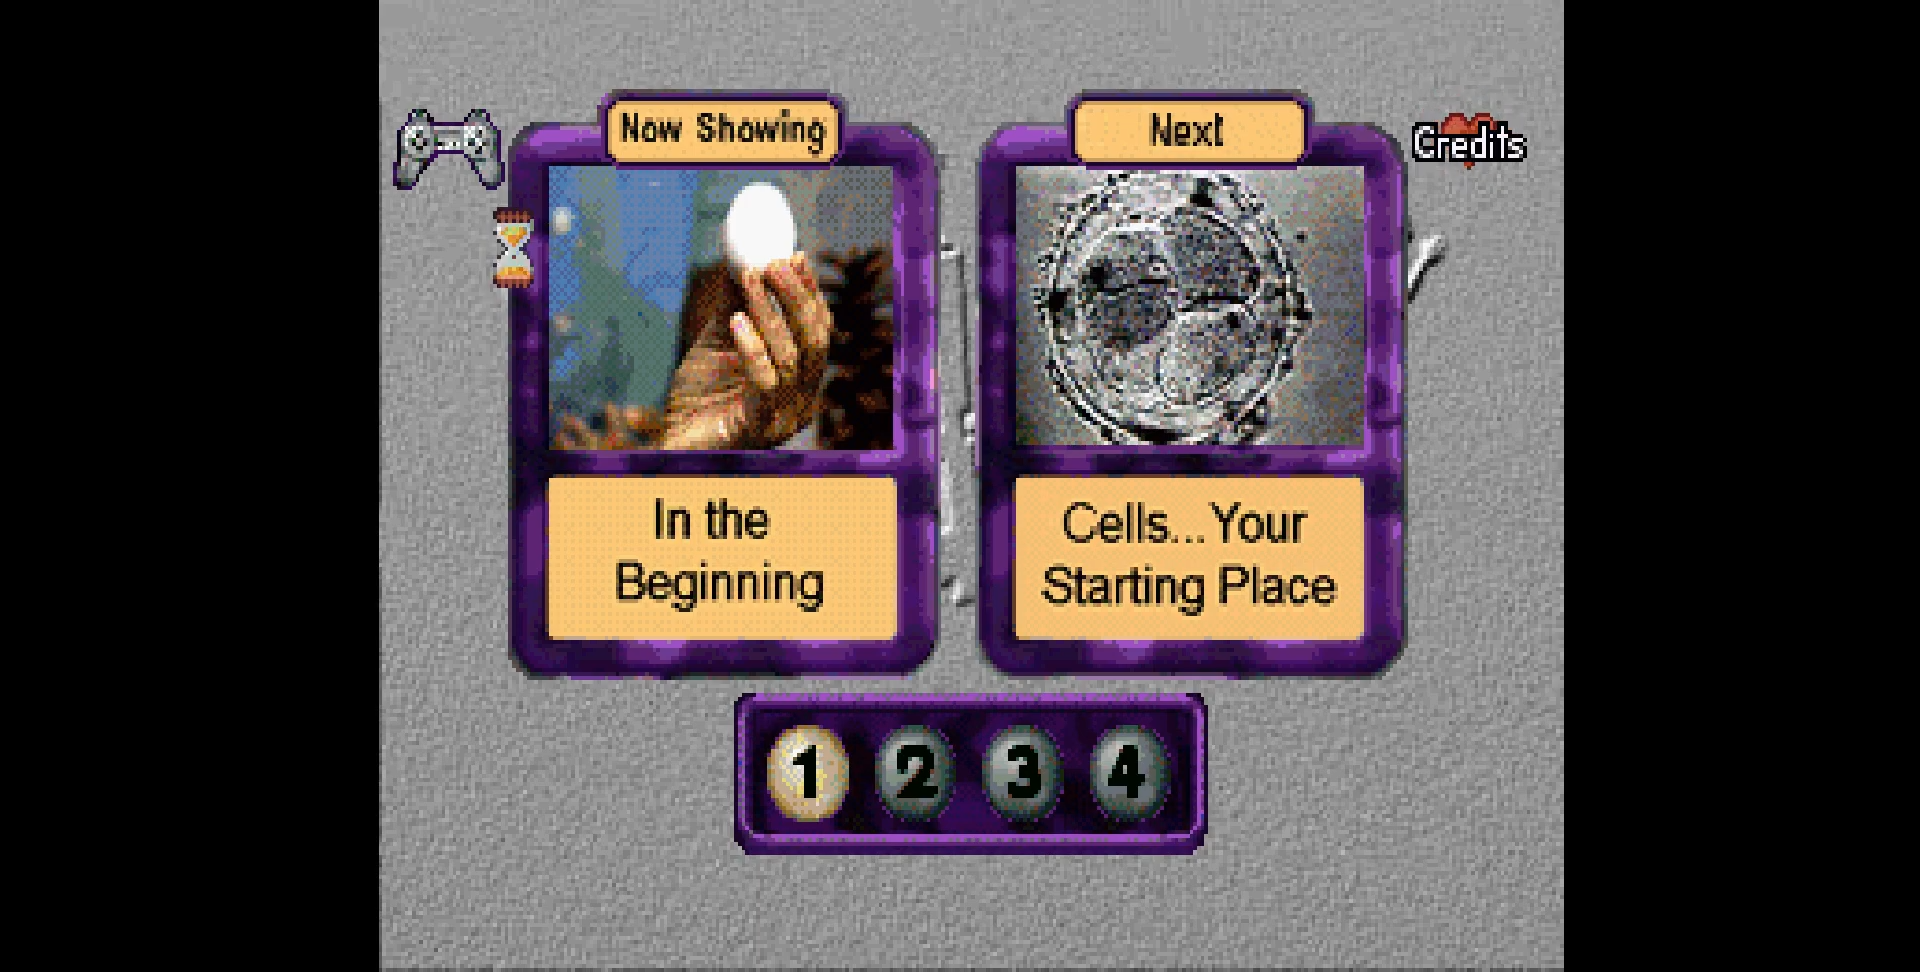
\includegraphics[width=\linewidth]{Games/HeadtoToe/Images/HeadToToe1Image1.png}
        \caption{Head To Toe 1 - Screenshot 1}
    \end{subfigure}
    \begin{subfigure}{0.45\textwidth}
        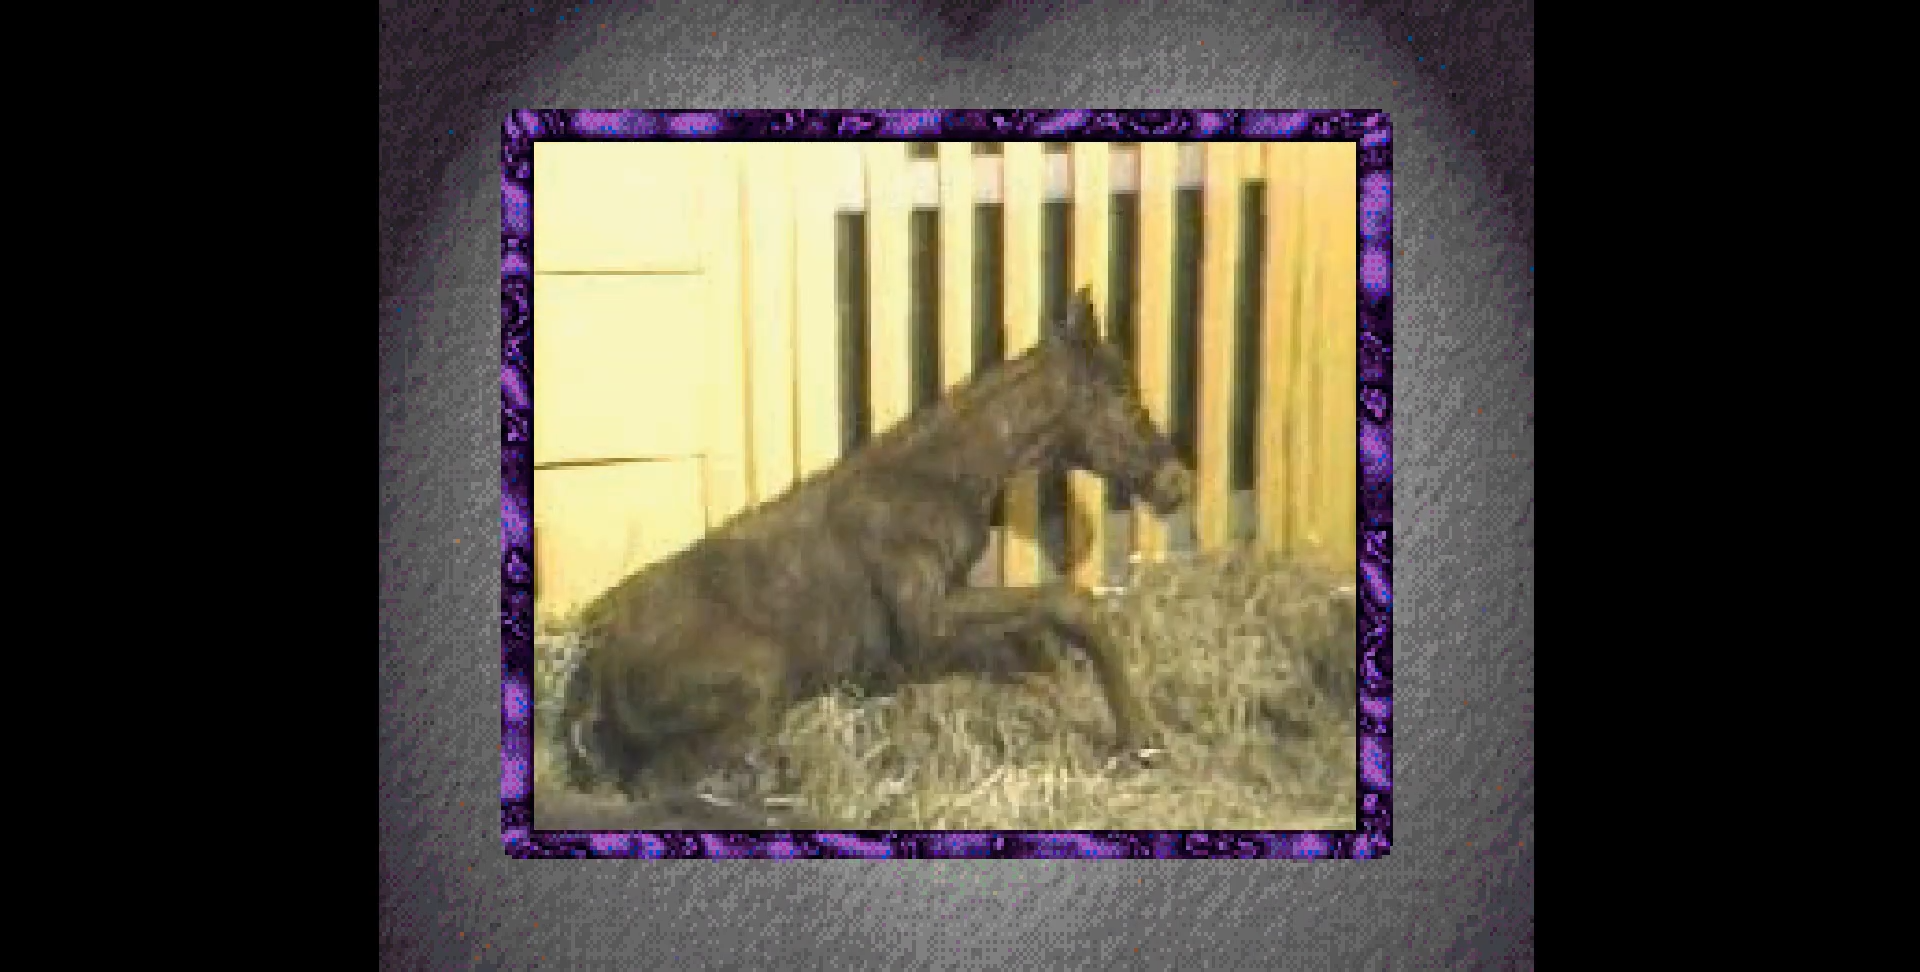
\includegraphics[width=\linewidth]{Games/HeadtoToe/Images/HeadToToe1Image2.png}
        \caption{Head To Toe 1 - Screenshot 2}
    \end{subfigure}

    \begin{subfigure}{0.45\textwidth}
        \centering
        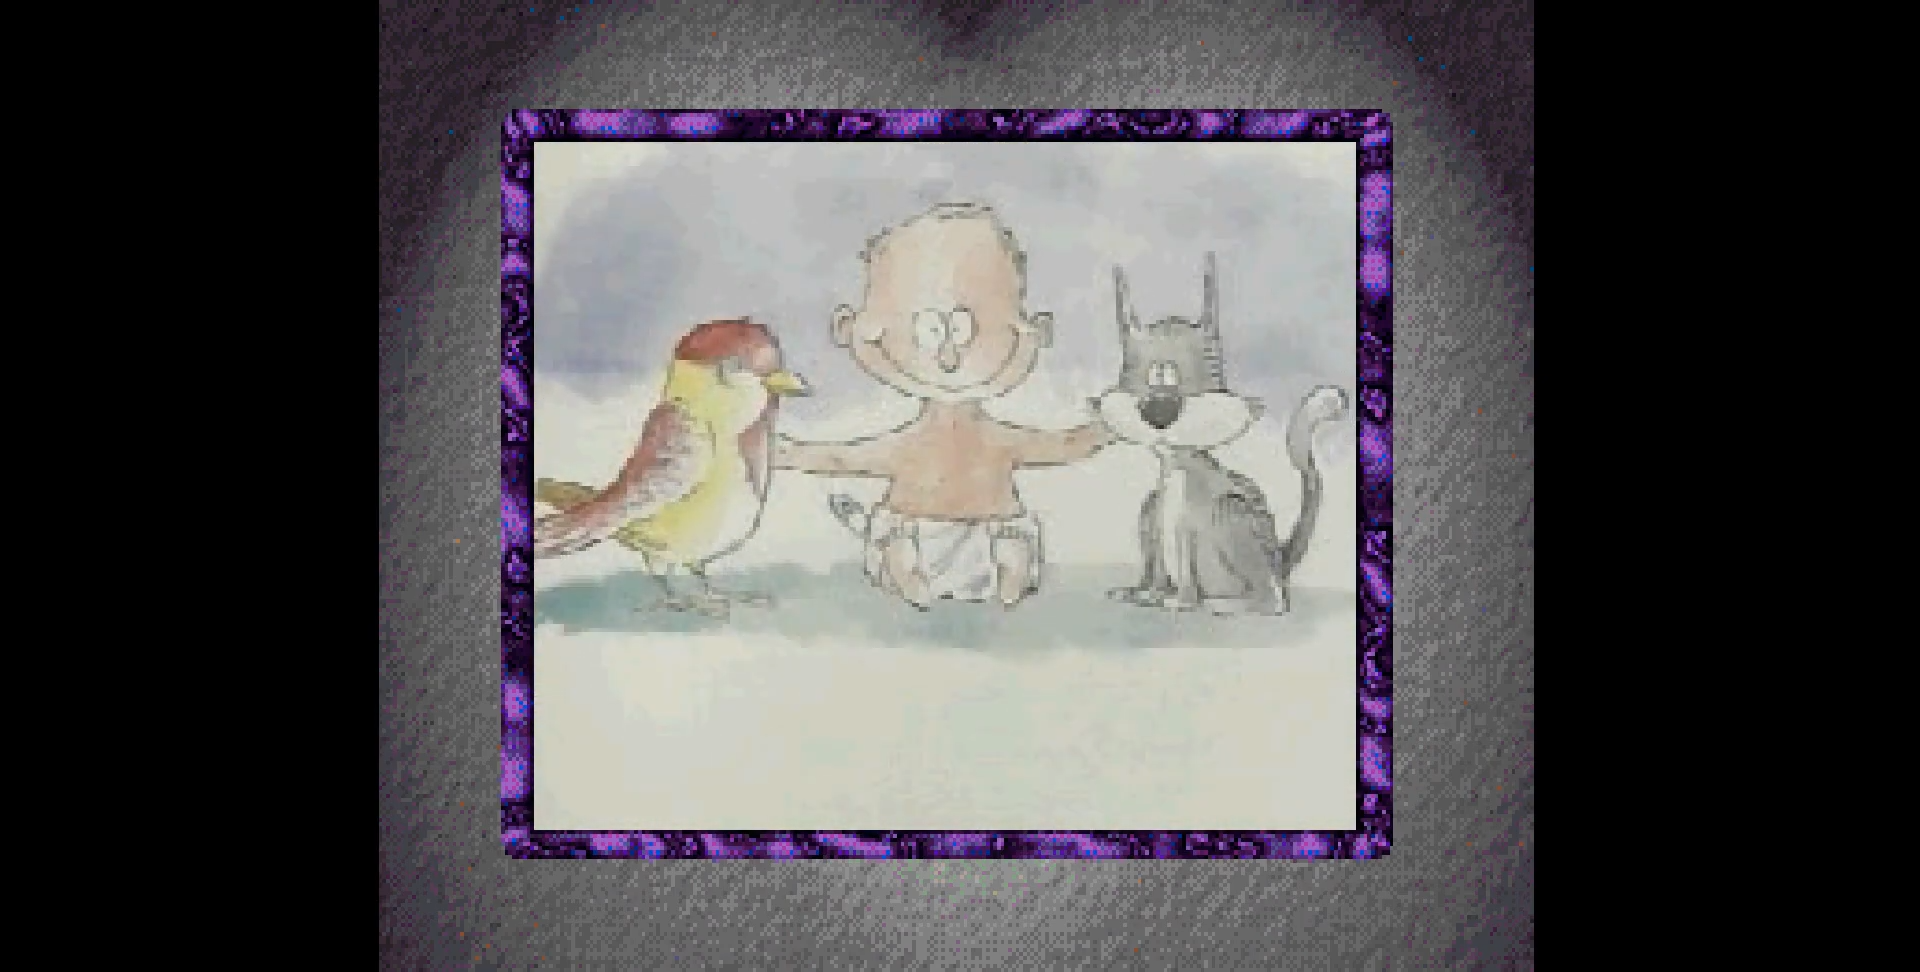
\includegraphics[width=\linewidth]{Games/HeadtoToe/Images/HeadToToe1Image3.png}
        \caption{Head To Toe 1 - Screenshot 3}
    \end{subfigure}
    \begin{subfigure}{0.45\textwidth}
        \centering
        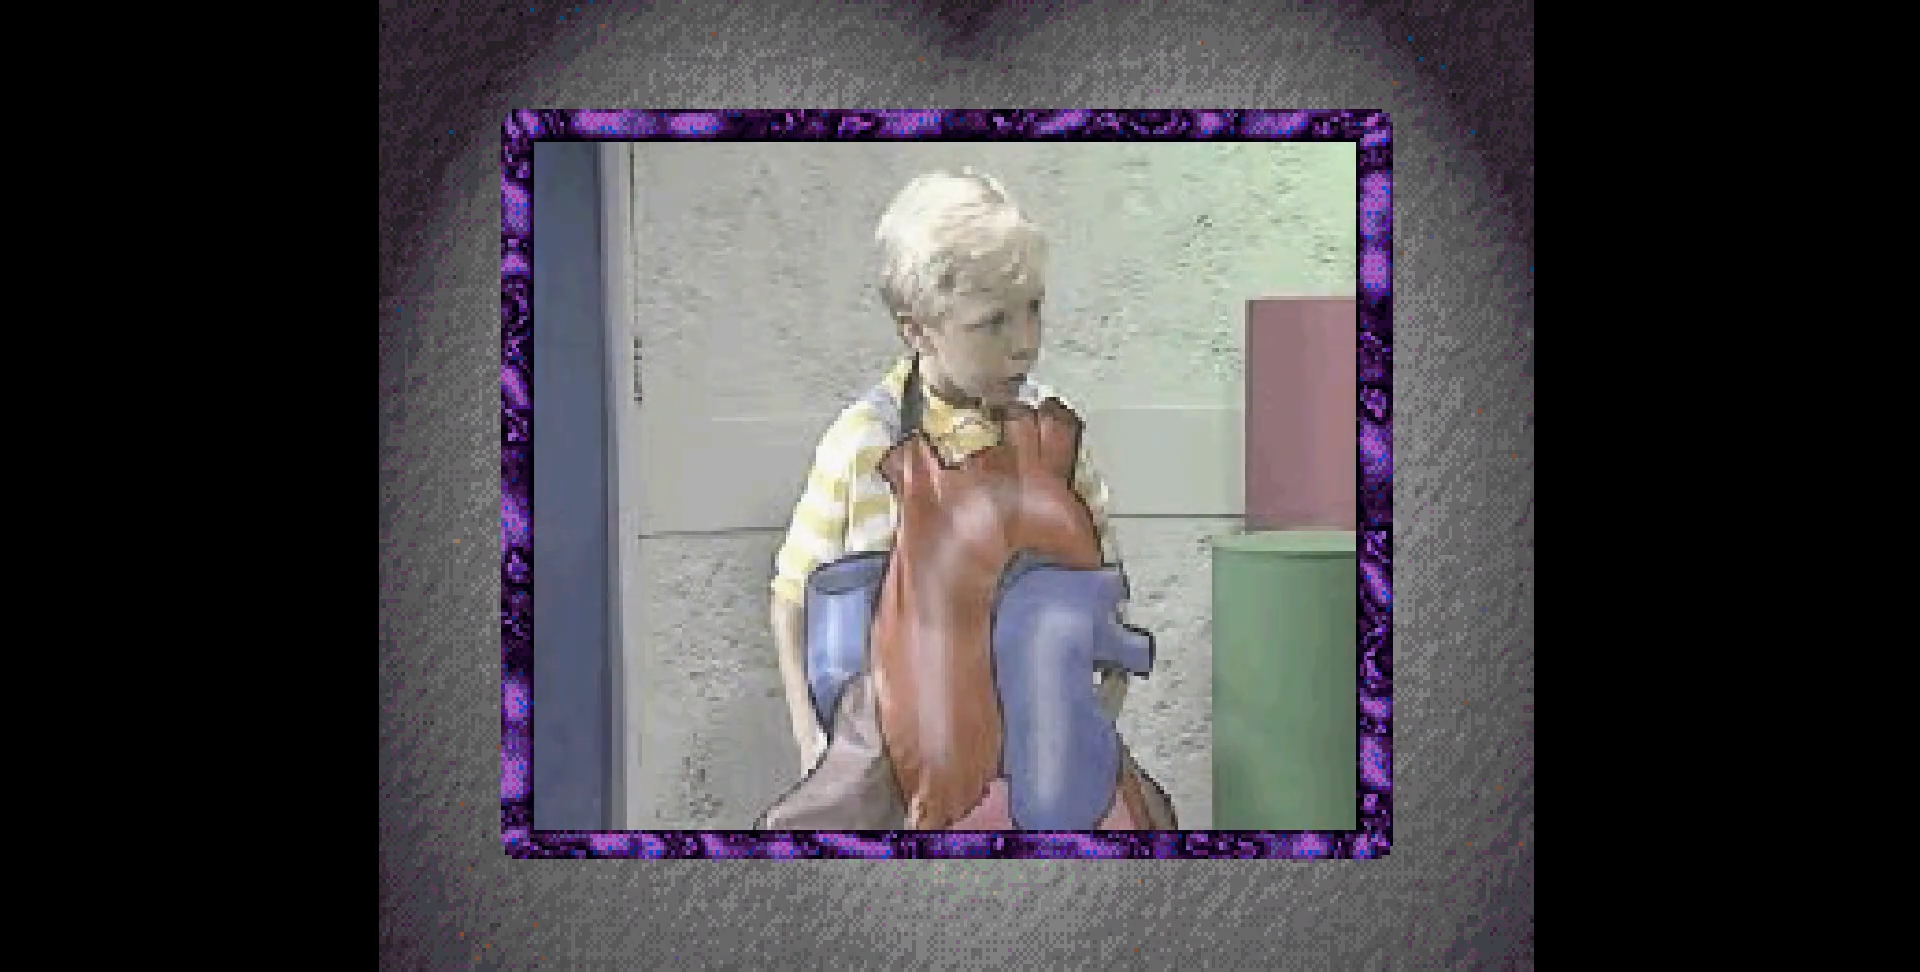
\includegraphics[width=\linewidth]{Games/HeadtoToe/Images/HeadToToe1Image4.png}
        \caption{Head To Toe 1 - Screenshot 4}
    \end{subfigure}
    \caption{Screenshots from Head To Toe 1}
\end{figure}